\documentclass[11pt,a4paper]{article}
\usepackage[utf8]{inputenc}  % .tex chars encoding
\usepackage[T1]{fontenc}     % .pdf chars encoding
\usepackage[italian]{babel}  % translations
\usepackage{amsmath}         % math symbols
\usepackage{amsfonts}        % extended math symbols
\usepackage{amssymb}         % other math symbols
\usepackage{hyperref}        % hyperref
\usepackage{graphicx}        % images
\usepackage{float}           % float options

% Macros
% ======
\newcommand*{\wix}{Wix}
\newcommand*{\wixcom}{wix.com}
\newcommand*{\wixcome}{\emph{\wixcom{}}}

% Configs
% =======

% Path relative to the main .tex file 
\graphicspath{ {./img/} }

\author{Luca Parolari}
\title{Web Information Management\\ \large Analisi di usabilità del sito web \wixcom{}}

% Document
% ========

\begin{document}

\maketitle

\clearpage
\tableofcontents

\clearpage

\section{Introduzione}
\label{sec:intro}

Questo documento si prefigge lo scopo di fornire un'analisi di
usabilità del sito web \href{https://wix.com}{\wixcom{}}. Il sito web è
stato analizzato nel periodo di gennaio 2021.

\begin{figure}[h]
  \centering
  
\includegraphics[width=0.25\textwidth]{wix-logo}
  \caption{Logo di \wix{}}
  \label{fix:wix-logo}
\end{figure}

\wix{} promuove il suo prodotto principale: un site builder fruibile da
tutti gli utenti sia con che senza conoscenza informatica. I suoi
obiettivi principali sono rendere semplice, immediata, user-friendly e
gratuita la manutenzione del proprio sito web online offrendo
strumenti integrati nel site builder per costruire e modificare blog,
e-commerce e siti vetrina.

\section{Analisi preliminare}
\label{sec:preliminary-analysis}

\subsection{Contesto}
\label{subsec:context}

\wix{}, in linea generale, è un site builder. Un site builder è uno
strumento software che tipicamente permette la costruzione di siti web
senza (o quasi) scrivere del codice
manualmente.\footnote{\url{https://en.wikipedia.org/wiki/Website_builder}}.
I
site builder si distinguono in due macro categorie: \emph{online} site
builder, dove lo strumento è fornito in cloud ed è gestito
privatamente dal provider che offre il servizio e lo spazio dove
hostare il proprio sito web e \emph{offline} site builder dove invece
lo strumento può essere eseguito sul computer e genera le pagine del
sito che possono poi essere distribuite su un qualunque web hosting.

\wix{} rientra chiaramente nella prima categoria: l'output generato
dal sitebuilder di \wix{} non può essere esportato su altri
provider. Questo rappresenta infatti il core-business di \wix{}: un
servizio di hosting con un grandissimo valore aggiungo, ovvero il site
builder. 

\subsection{Nome del sito}
\label{subsec:site-name}

Il nome \wix{} è ben fatto e segue delle regole ben precise. Esso infatti è

\begin{itemize}
  \item unico;
  \item corto a tal punto che è composto dal minimo numero di lettere
    per creare un nome orecchiabile;
  \item facile da memorizzare e da scrivere, anche se presenta lettere
    come la \emph{w} e la \emph{x} provenienti dall'afabeto
    internazionale e non originariamente presenti nell'afabeto
    italiano. Quest'ultime però sono ormai state sdoganate e tutti ne
    conoscono l'esistenza;
  \item seguito dal dominio ``.com'', molto famoso e facile da
    indovinare anche se non memorizzato;
\end{itemize}

Inoltre, il nome \wix{} risulta correttamente registrato (controllo eseguito su \href{https://www3.wipo.int/branddb/en/}{WIPO
  Global Brand Database}).


\section{Homepage}
\label{sec:homepage-analysis}

Nella sezione \ref{subsec:homepage-description} viene descritta la
homepage screen per screen dato lo sviluppo verticale della pagina,
mentre in \ref{subsec:homepage-the-six-ws} viene argomentata le
gestione delle informazioni per quanto riguarda i sei assi informativi
della pagina web.

\subsection{Descrizione generale}
\label{subsec:homepage-description}

Dall'URL \url{https://wix.com} si accede alla homapage del sito
\wix{}. La figura \ref{fig:homepage-01} mostra la schermata più
importante del sito web, ovvero quella visibile senza alcuno scroll e
quindi accessibile da tutti gli utenti.

L'entry point di questa pagina è il logo di \wix{} che occupa, con del
testo, esattamente la posizione in alto a sinistra della pagina. Il
menu poi prosegue con alcune voci per navigare il sito ed un pulsante
\textit{Accedi}, che probabilmente viene utilizzato dagli utenti
ricorrenti per accedere al proprio account. L'unica parte veramente
informativa della pagina è il titolo nel mezzo dell'immagine: ``Crea
il tuo sito web professionale'', che lascia intuire l'obiettivo del
sito ma non lo esplicita completamente. Dal punto di vista informativo
questa pagina è molto povera e sicuramente non riesce a soddisfare le
richieste dell'utente, il quale vorrebbe per lo meno capire in che
sito web è capitato.

Il click sul pulsante \textit{Inizia} non porta ad ulteriori
informazioni, bensì ad una pagina di accesso/registrazione: siamo di
fronte al problema della registrazione prematura, in quanto in questa
fase, un utente nuovo, non ha ancora capito lo scopo del sito.

\begin{figure}[H]
  \centering
  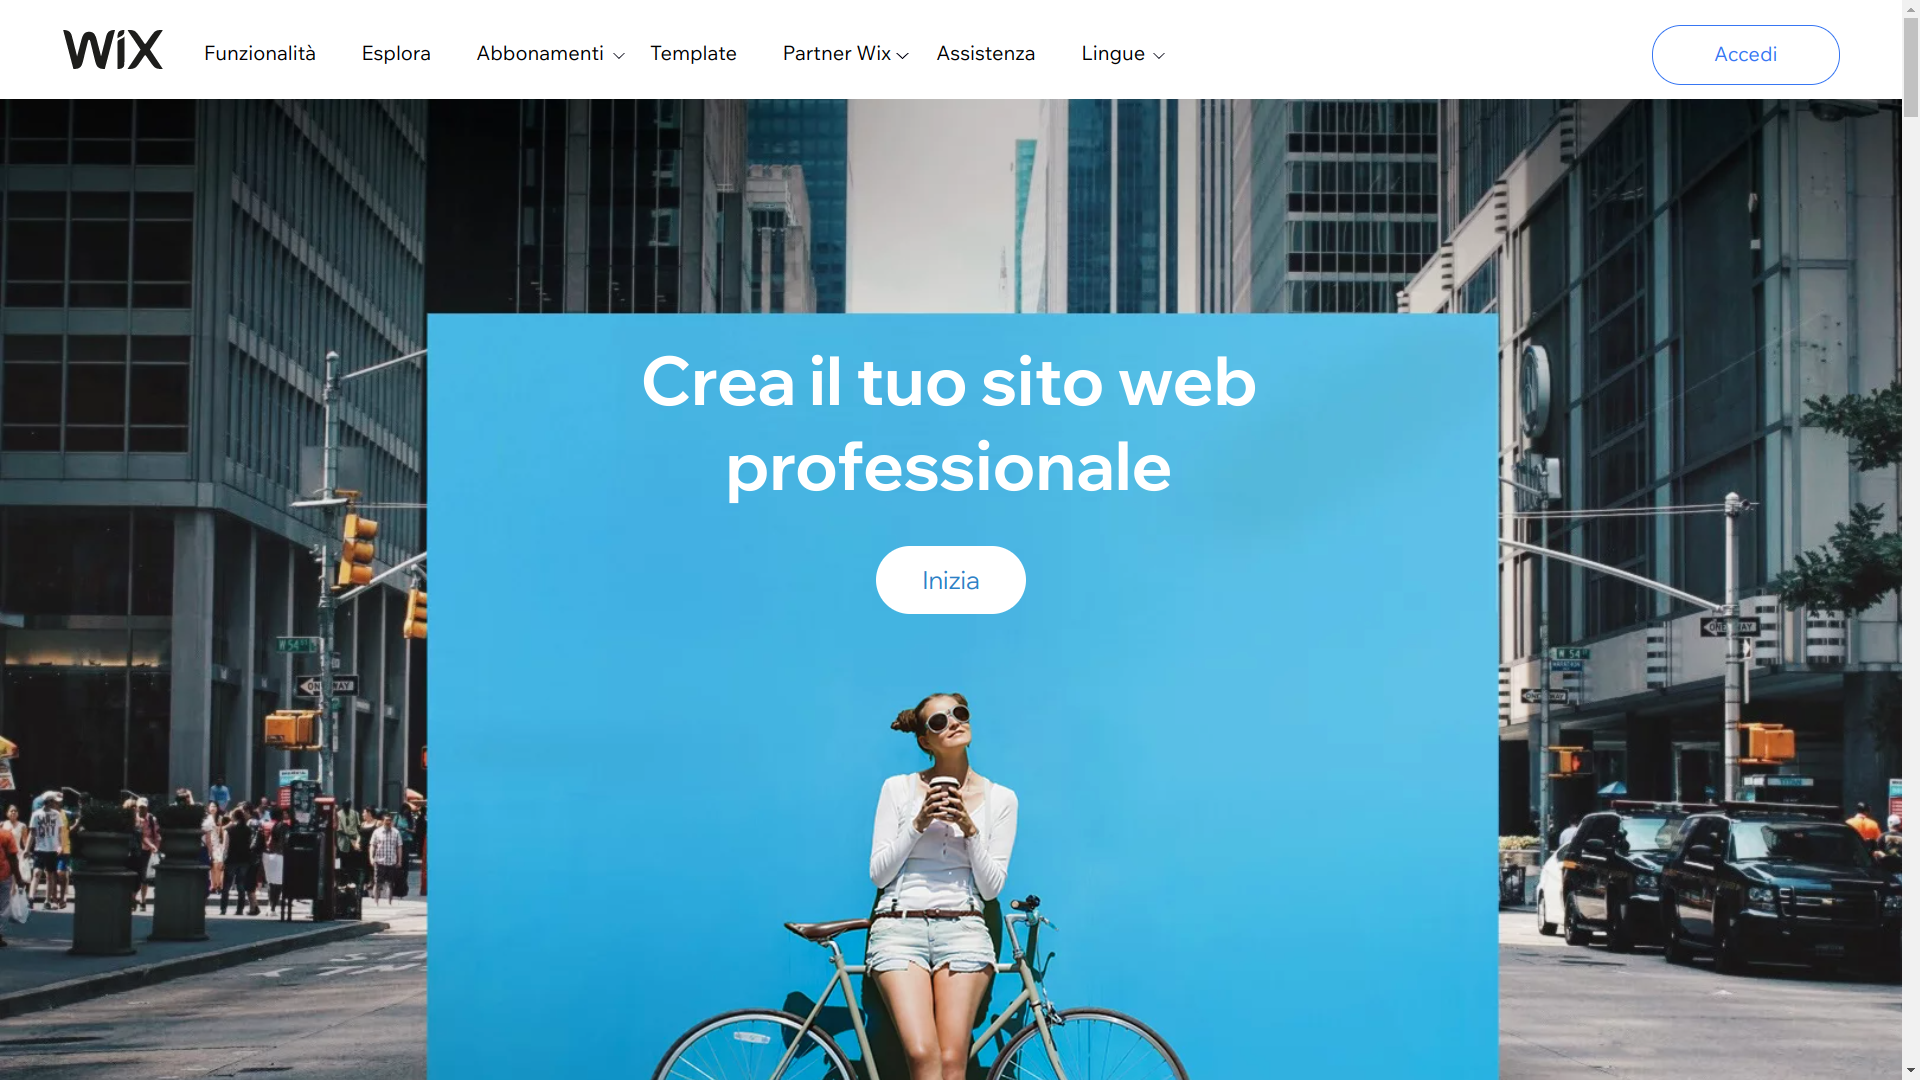
\includegraphics[width=1\textwidth]{img/homepage-01.png}
  \caption{Homepage (pt. 1)}
  \label{fig:homepage-01}
\end{figure}

Proseguendo con il primo scroll, la figura \ref{fig:homepage-02}
mostra la seconda schermata del sito web. Vi è un titolo molto
evocativo sulla sinistra ma comunque poco informativo, mentre il
paragrafo descrive meglio l'obiettivo di \wix{}. Il link
\textit{Inizia} porta ancora una volta alla pagina di registrazione
piuttosto che fornire altre informazioni. Per queste dobbiamo
scrollare.

\begin{figure}[H]
  \centering
  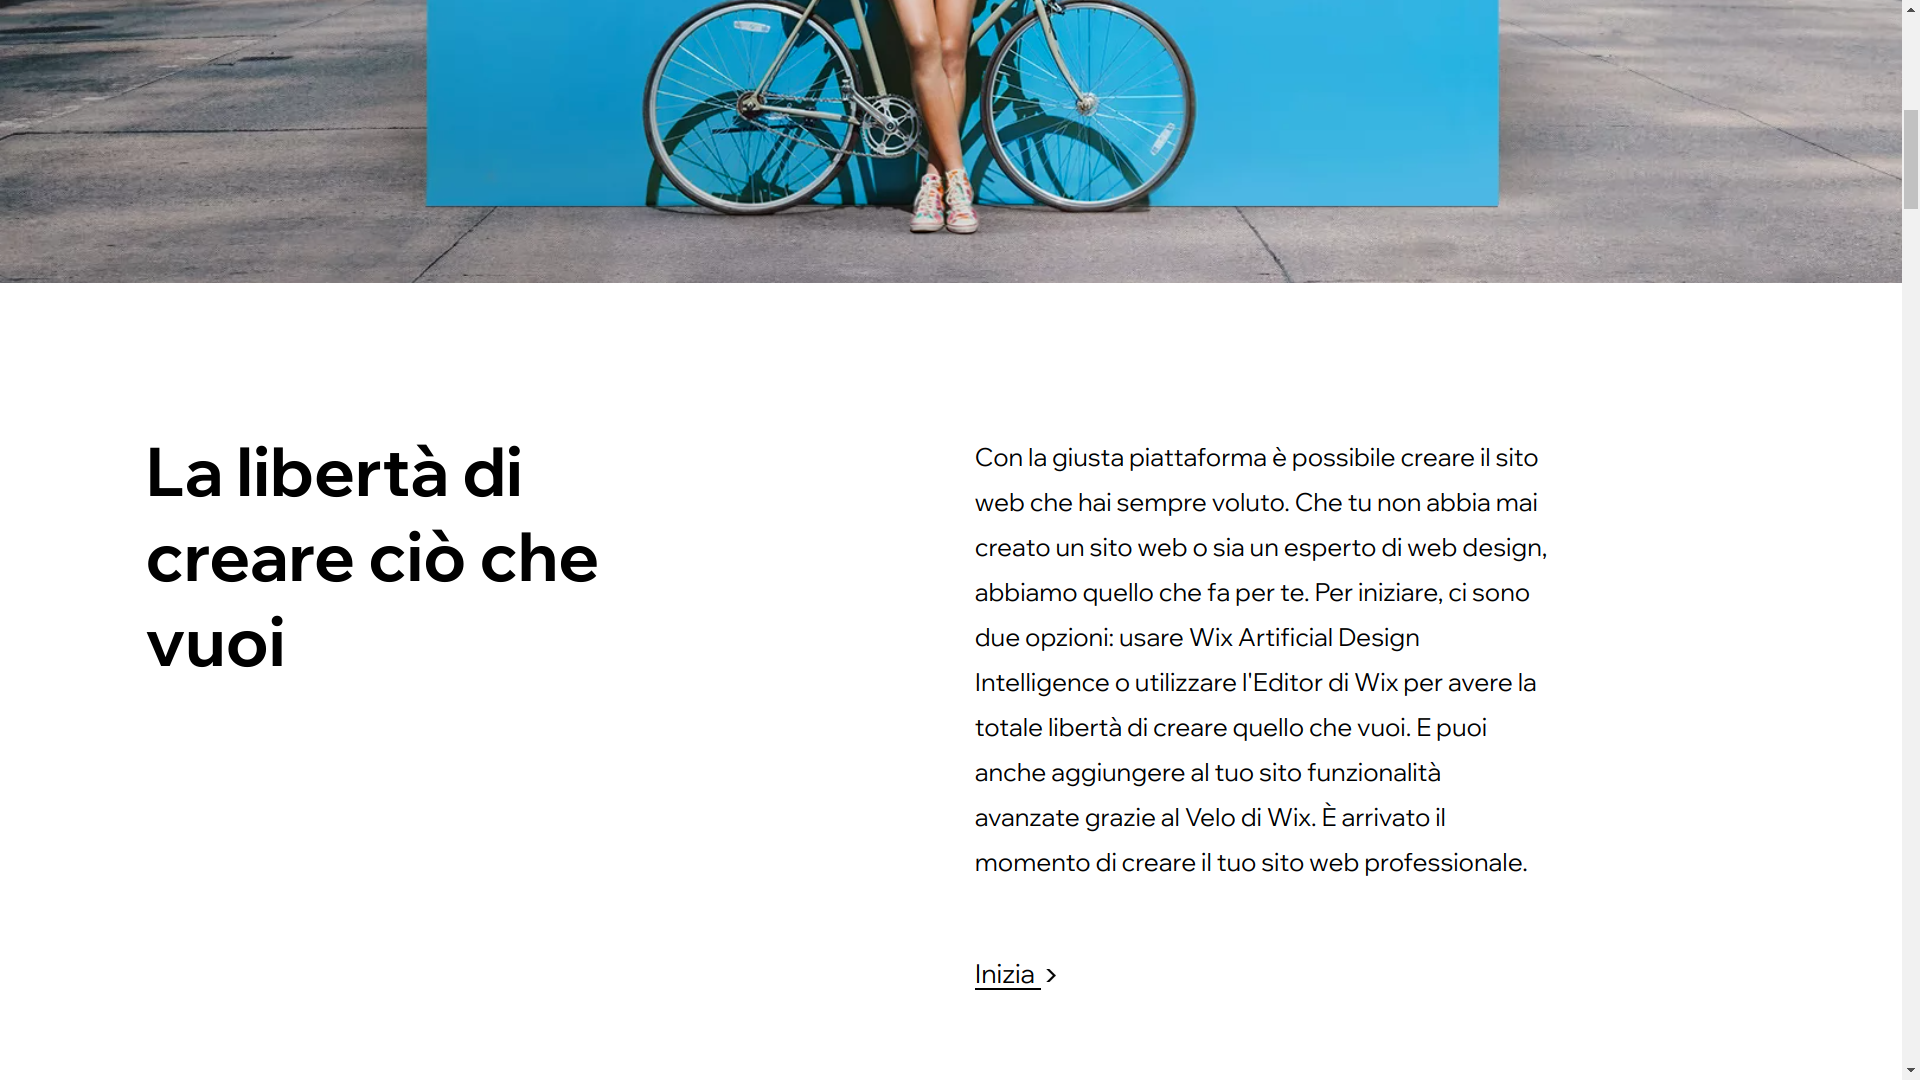
\includegraphics[width=1\textwidth]{img/homepage-02.png}
  \caption{Homepage (pt. 2)}
  \label{fig:homepage-02}
\end{figure}

Le immagini \ref{fig:homepage-03}, \ref{fig:homepage-04} e
\ref{fig:homepage-05} raffigurano le schermate della homepage dove vi
sono alcune informazioni sul prodotto presentato. I titoli non sono
del tutto chiari, ad esempio ``Velo'' e ``Wix ADI'' non restituiscono
all'utente un feedback immediato su quello che andrà a leggere, anche
se poi sono presenti dei sottotitoli indicano meglio di cosa si sta
parlando. 

Queste tre schermate, pur essendo molto belle visivamente sprecano non
poco spazio nell'illustrare le funzionalità del prodotto: le immagini
non sono sfruttate al massimo per enfatizzare il testo in quanto i box
separano concettualmente testo dall'immagine.

\begin{figure}[H]
  \centering
  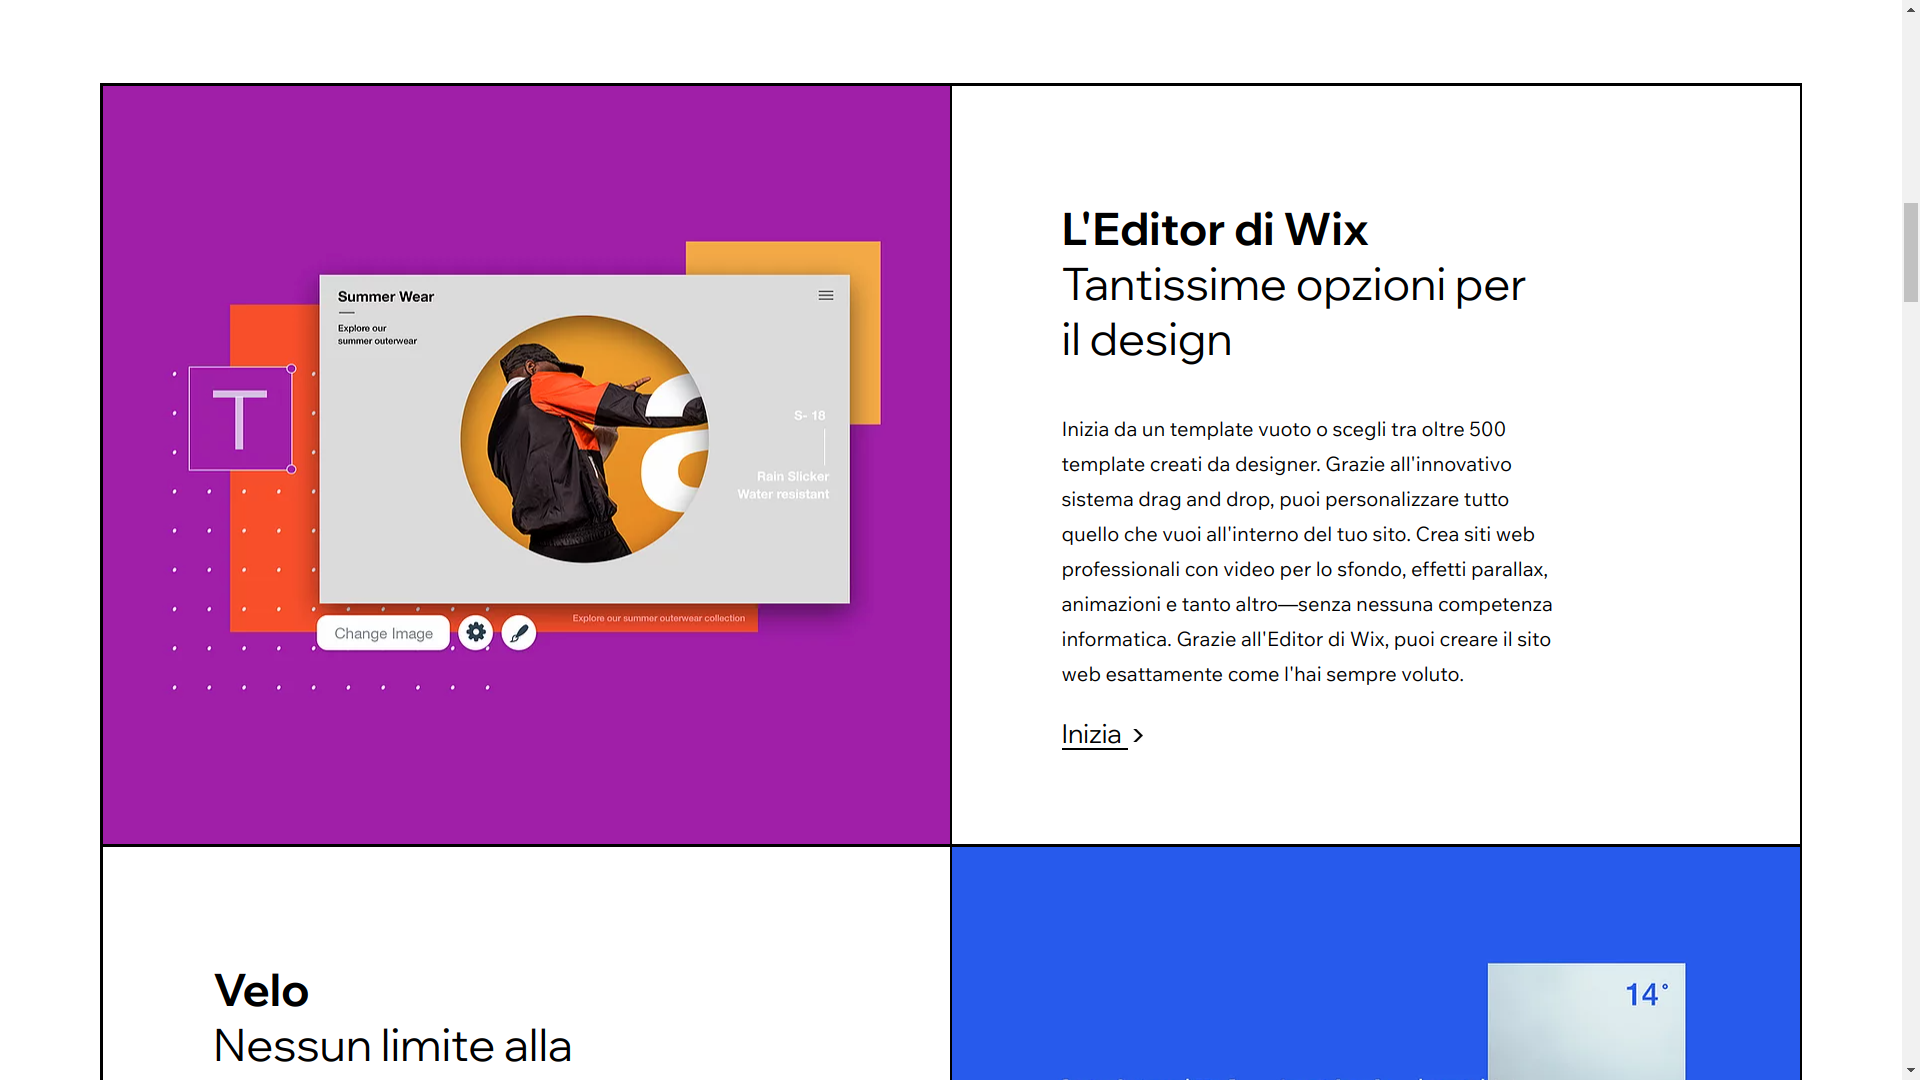
\includegraphics[width=1\textwidth]{img/homepage-03.png}
  \caption{Homepage (pt. 3)}
  \label{fig:homepage-03}
\end{figure}

\begin{figure}[H]
  \centering
  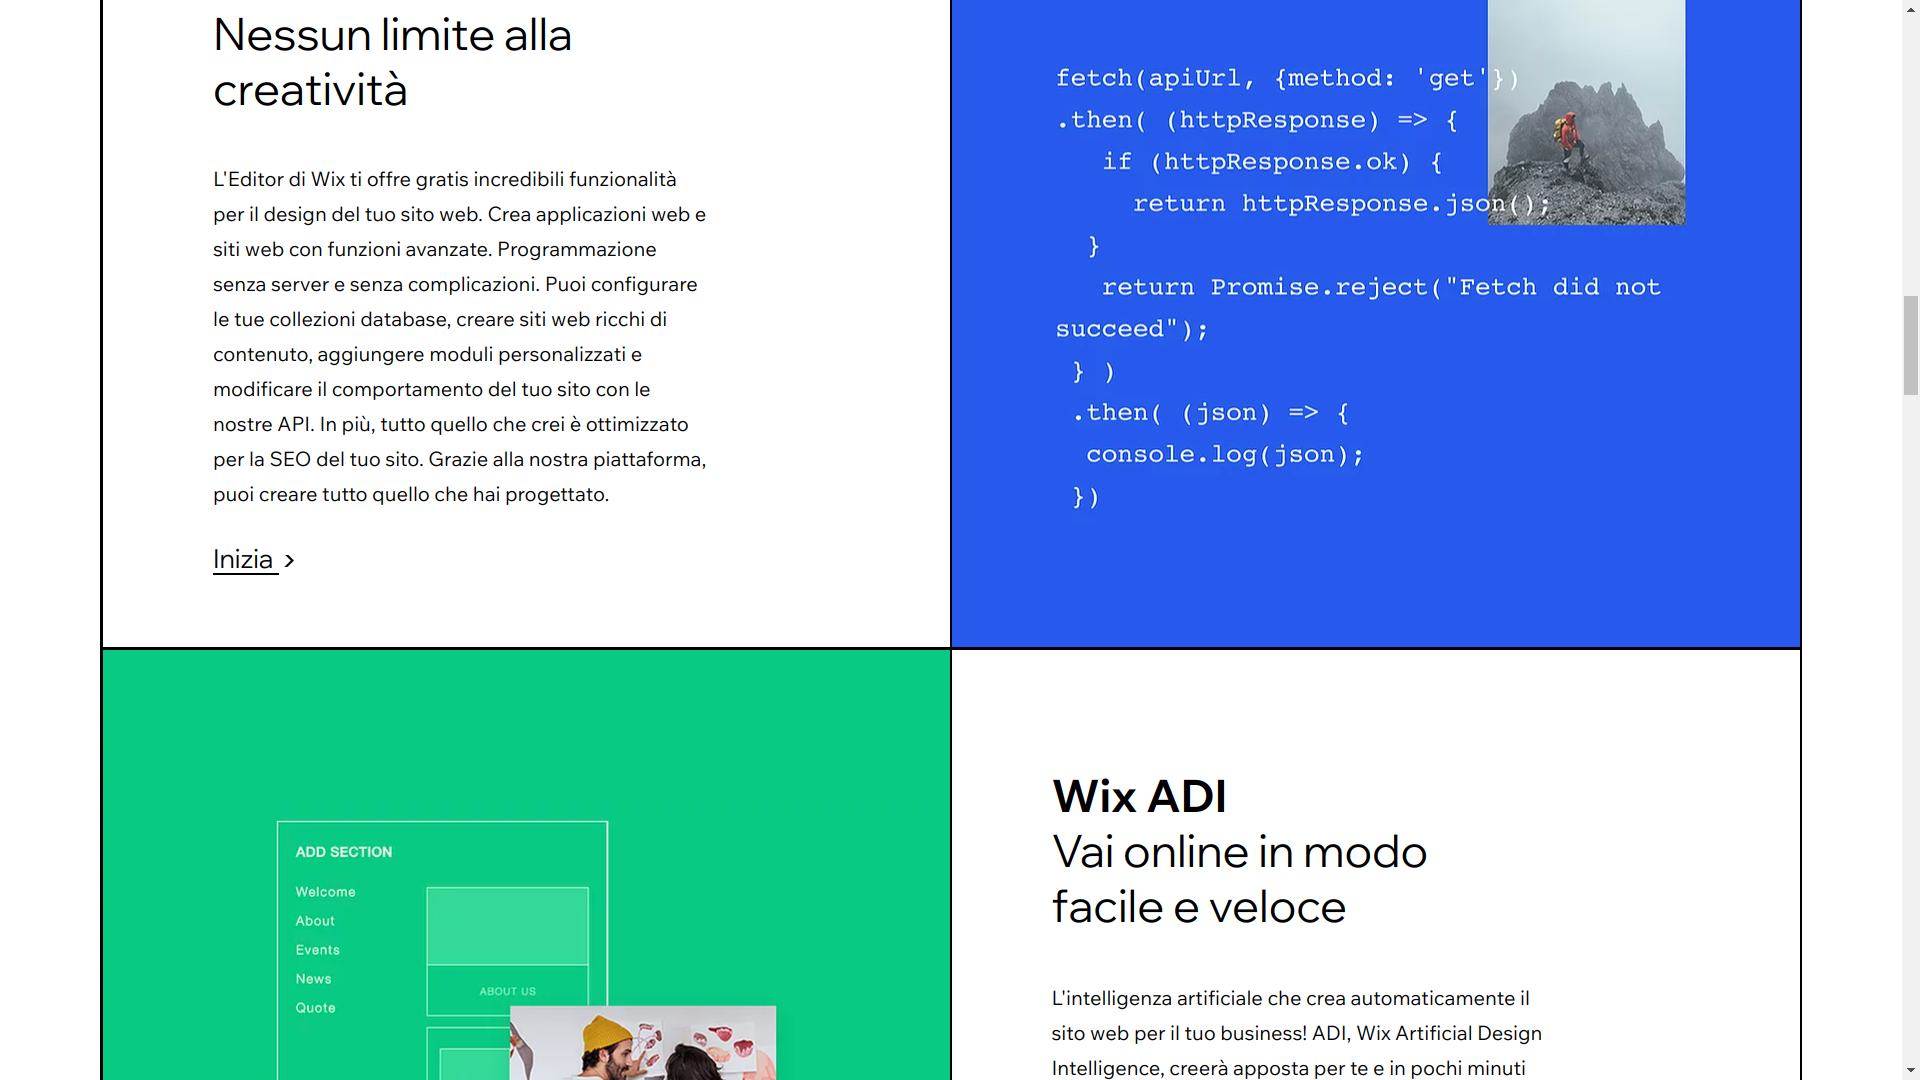
\includegraphics[width=1\textwidth]{img/homepage-04.png}
  \caption{Homepage (pt. 4)}
  \label{fig:homepage-04}
\end{figure}

\begin{figure}[H]
  \centering
  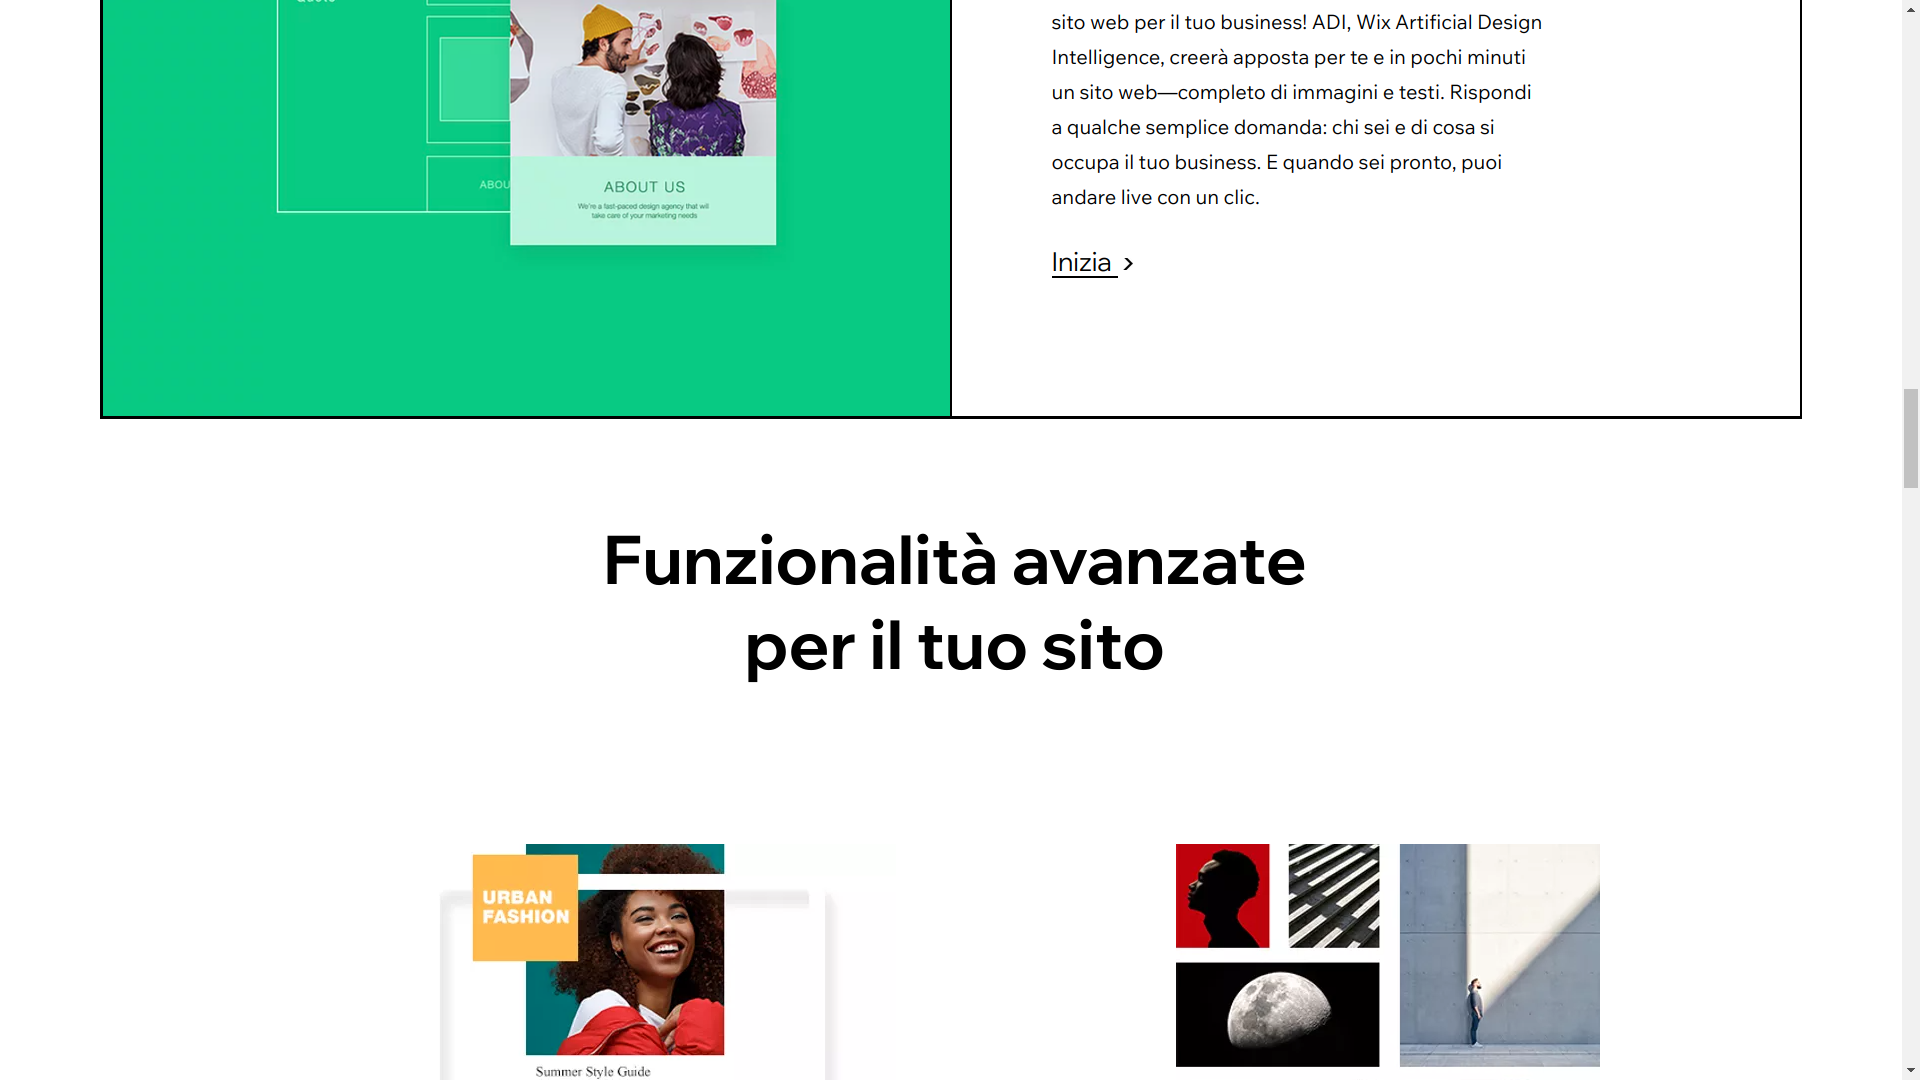
\includegraphics[width=1\textwidth]{img/homepage-05.png}
  \caption{Homepage (pt. 5)}
  \label{fig:homepage-05}
\end{figure}

La percentuale di utenti che continua ad essere presenti sul sito web
dopo quattro scroll è drasticamente ridotta, ma di fatto sono stati
presentati pochi contenuti, infatti il sito web continua con le
schermate \ref{fig:homepage-06} e \ref{fig:homepage-07}. In queste due
schermate vengono presentate altre funzionalità (avanzate) dello
strumento. Questi paragrafi sono concisi ed efficaci, inoltre sono
supportati da titoli che enfatizzano bene il concetto descritto. Anche
in questo caso però si spreca molto spazio con le immagini. La
presentazione delle caratteristiche inoltre è strutturata secondo uno
schema a griglia, e anche se gli elementi a schermo sono pochi, questa
distribuzione dei contenuti può generare confusione nell'utente dovuta
all'effetto \textit{random walk}.

\begin{figure}[H]
  \centering
  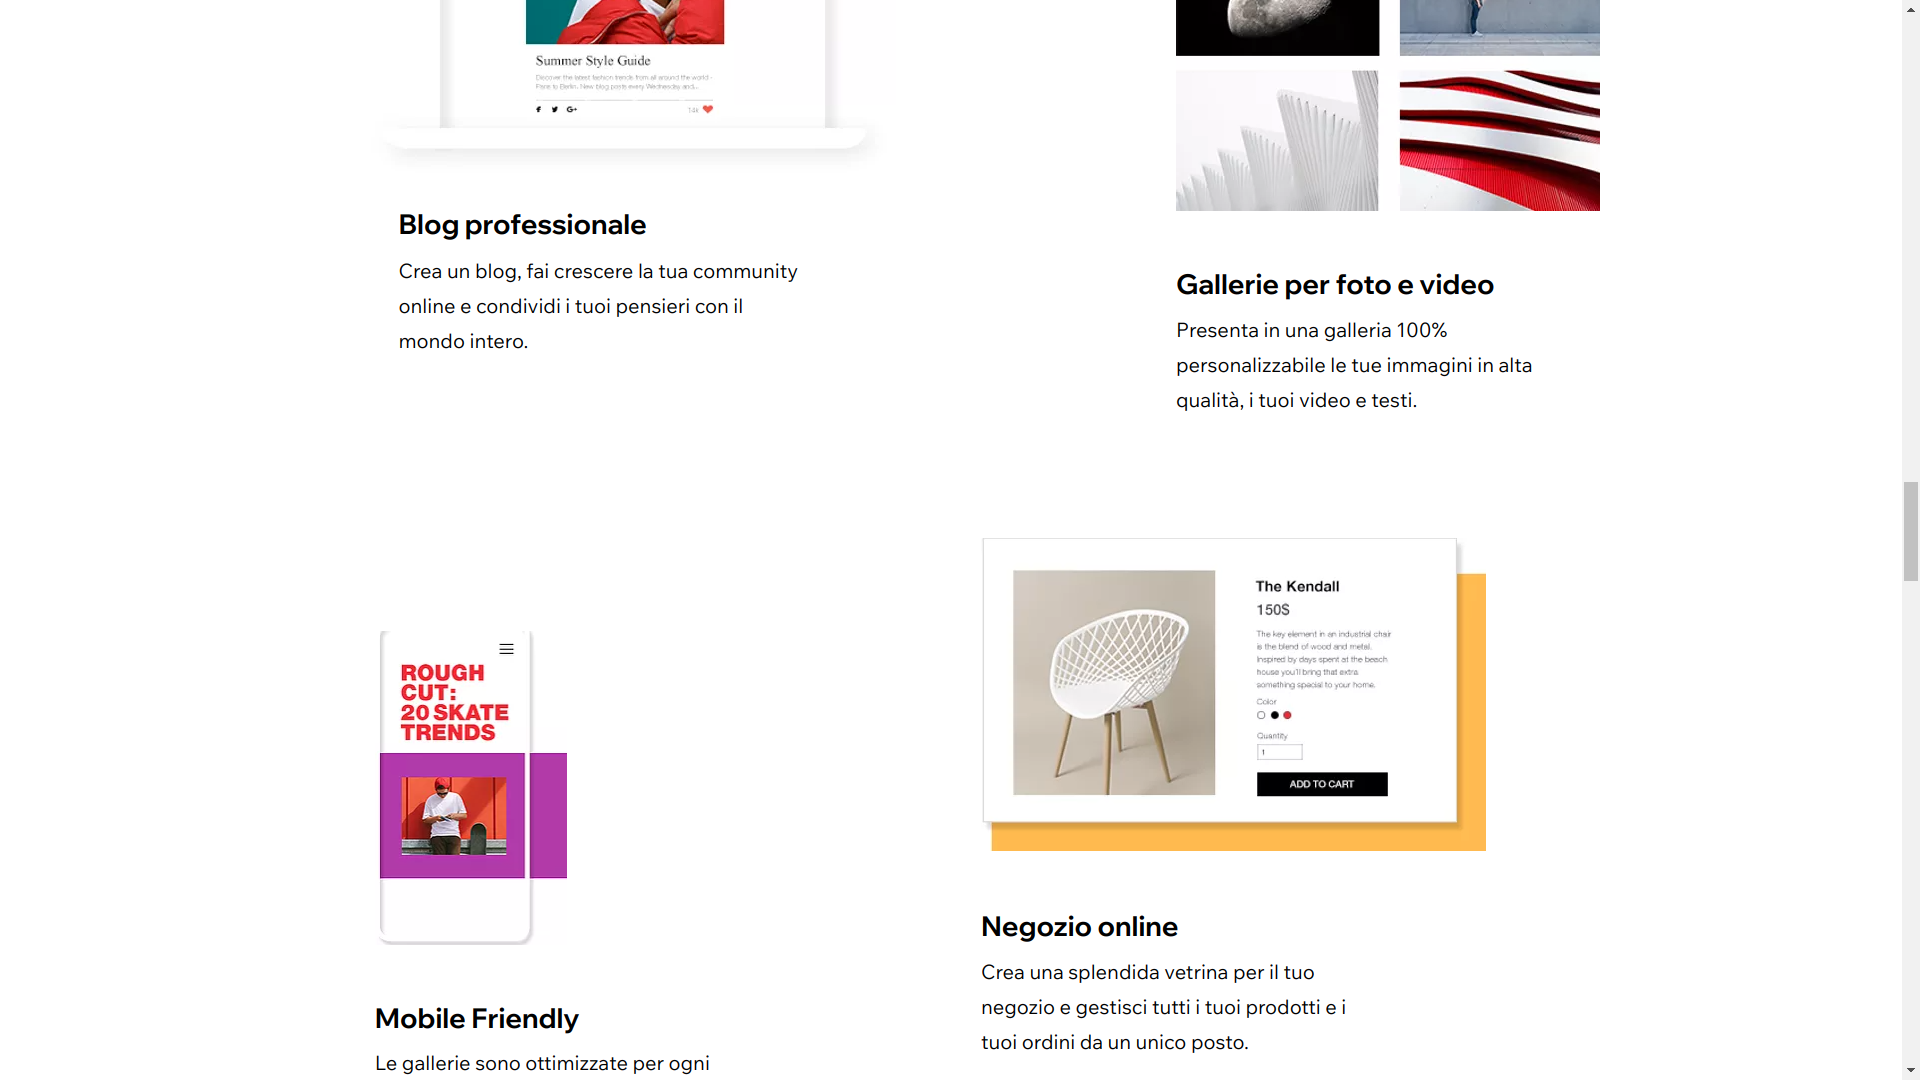
\includegraphics[width=1\textwidth]{img/homepage-06.png}
  \caption{Homepage (pt. 6)}
  \label{fig:homepage-06}
\end{figure}

\begin{figure}[H]
  \centering
  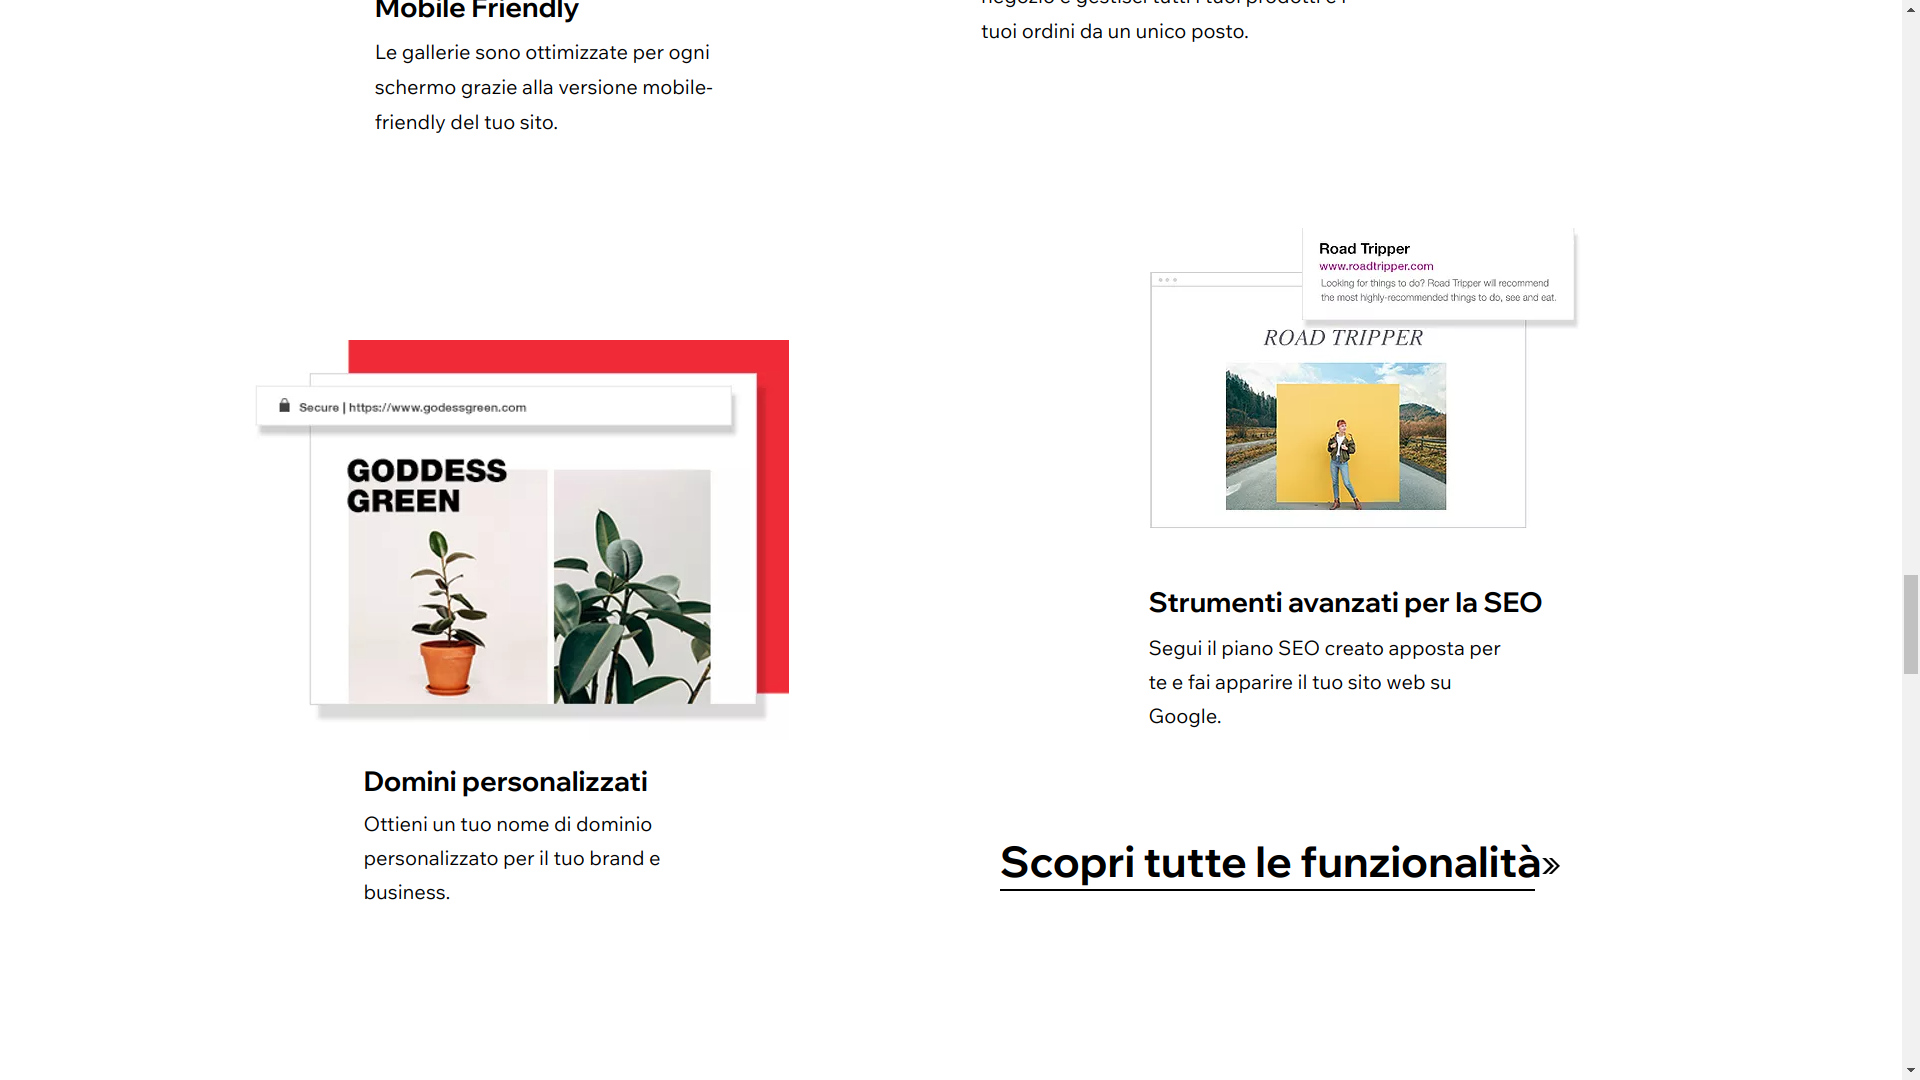
\includegraphics[width=1\textwidth]{img/homepage-07.png}
  \caption{Homepage (pt. 7)}
  \label{fig:homepage-07}
\end{figure}

Le schermate \ref{fig:homepage-08} e \ref{fig:homepage-09} illustrano
altre informazioni su \wix{}. In particolare viene esplicitata
l'utenza target, ovvero utenti con o senza conoscenza informatica e il
perché \wix{} è lo strumento da scegliere per costruire un sito web.

\begin{figure}[H]
  \centering
  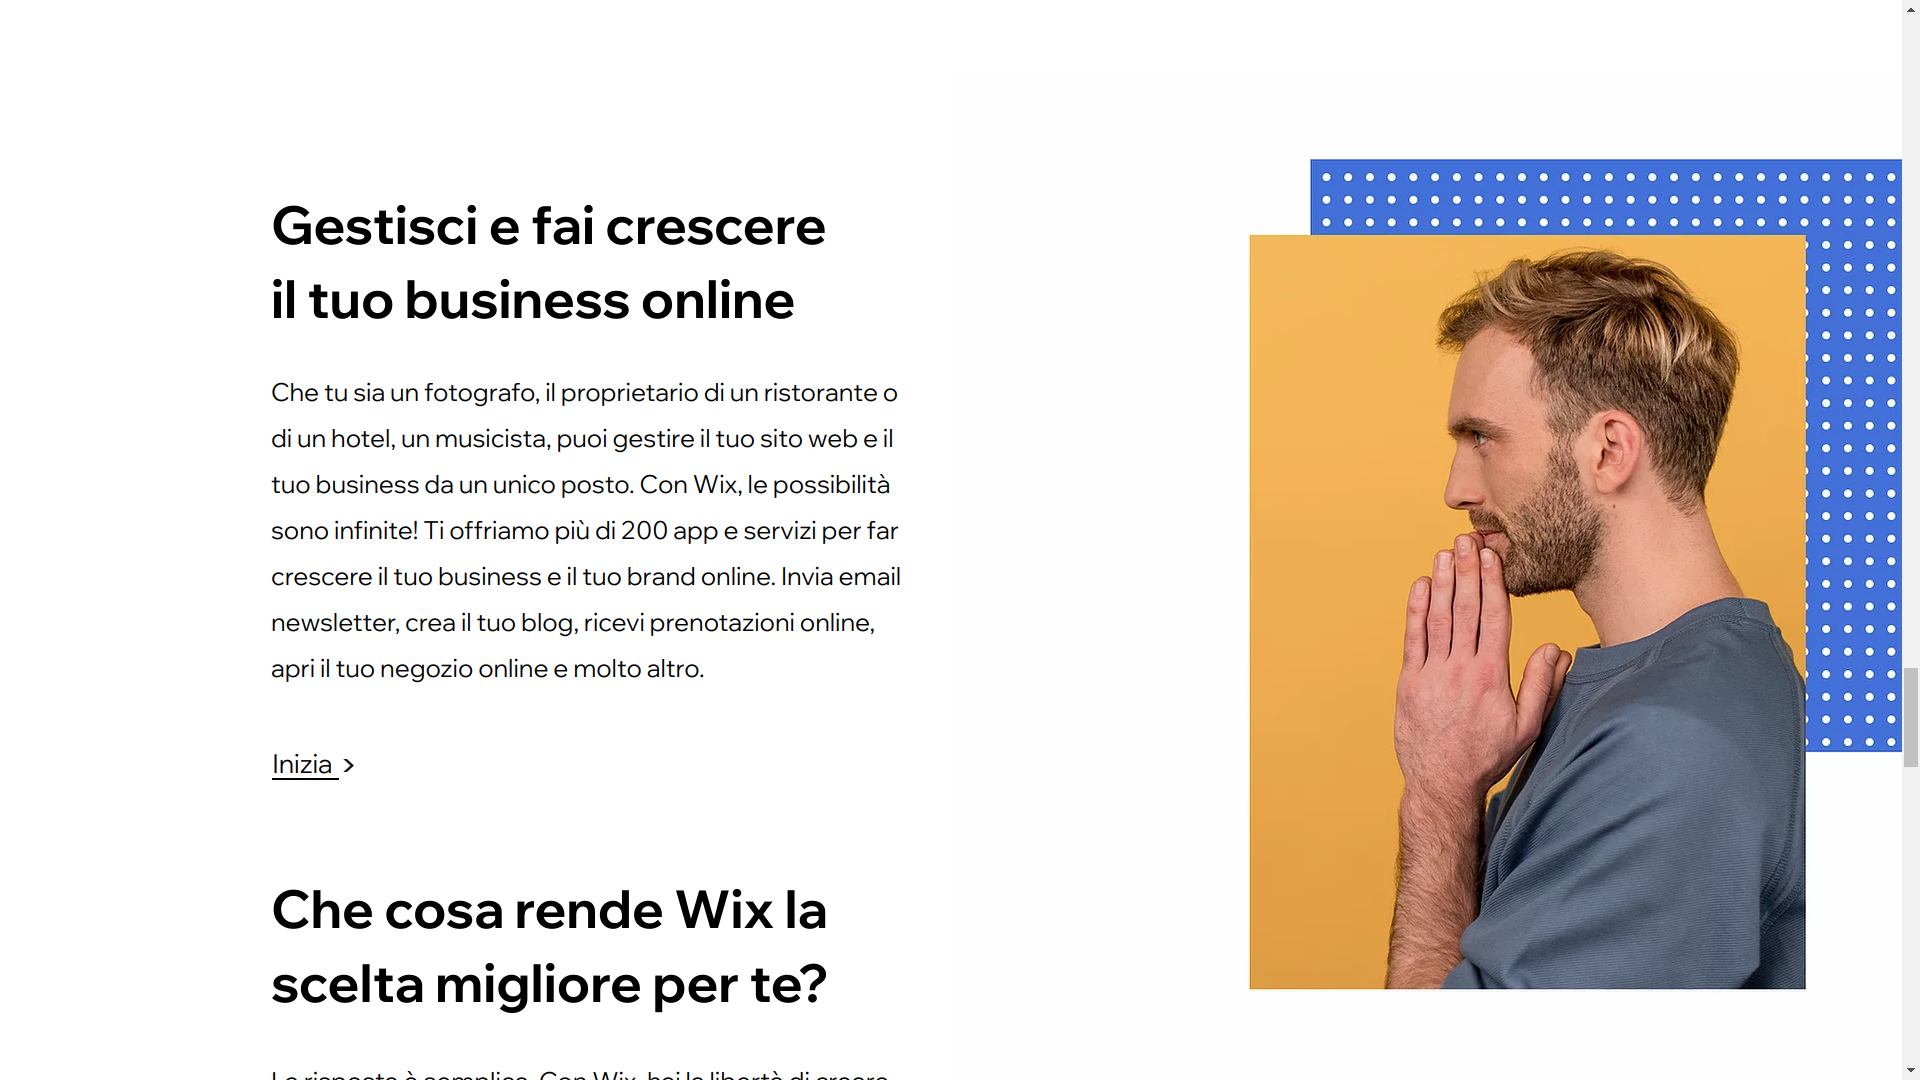
\includegraphics[width=1\textwidth]{img/homepage-08.png}
  \caption{Homepage (pt. 8)}
  \label{fig:homepage-08}
\end{figure}

\begin{figure}[H]
  \centering
  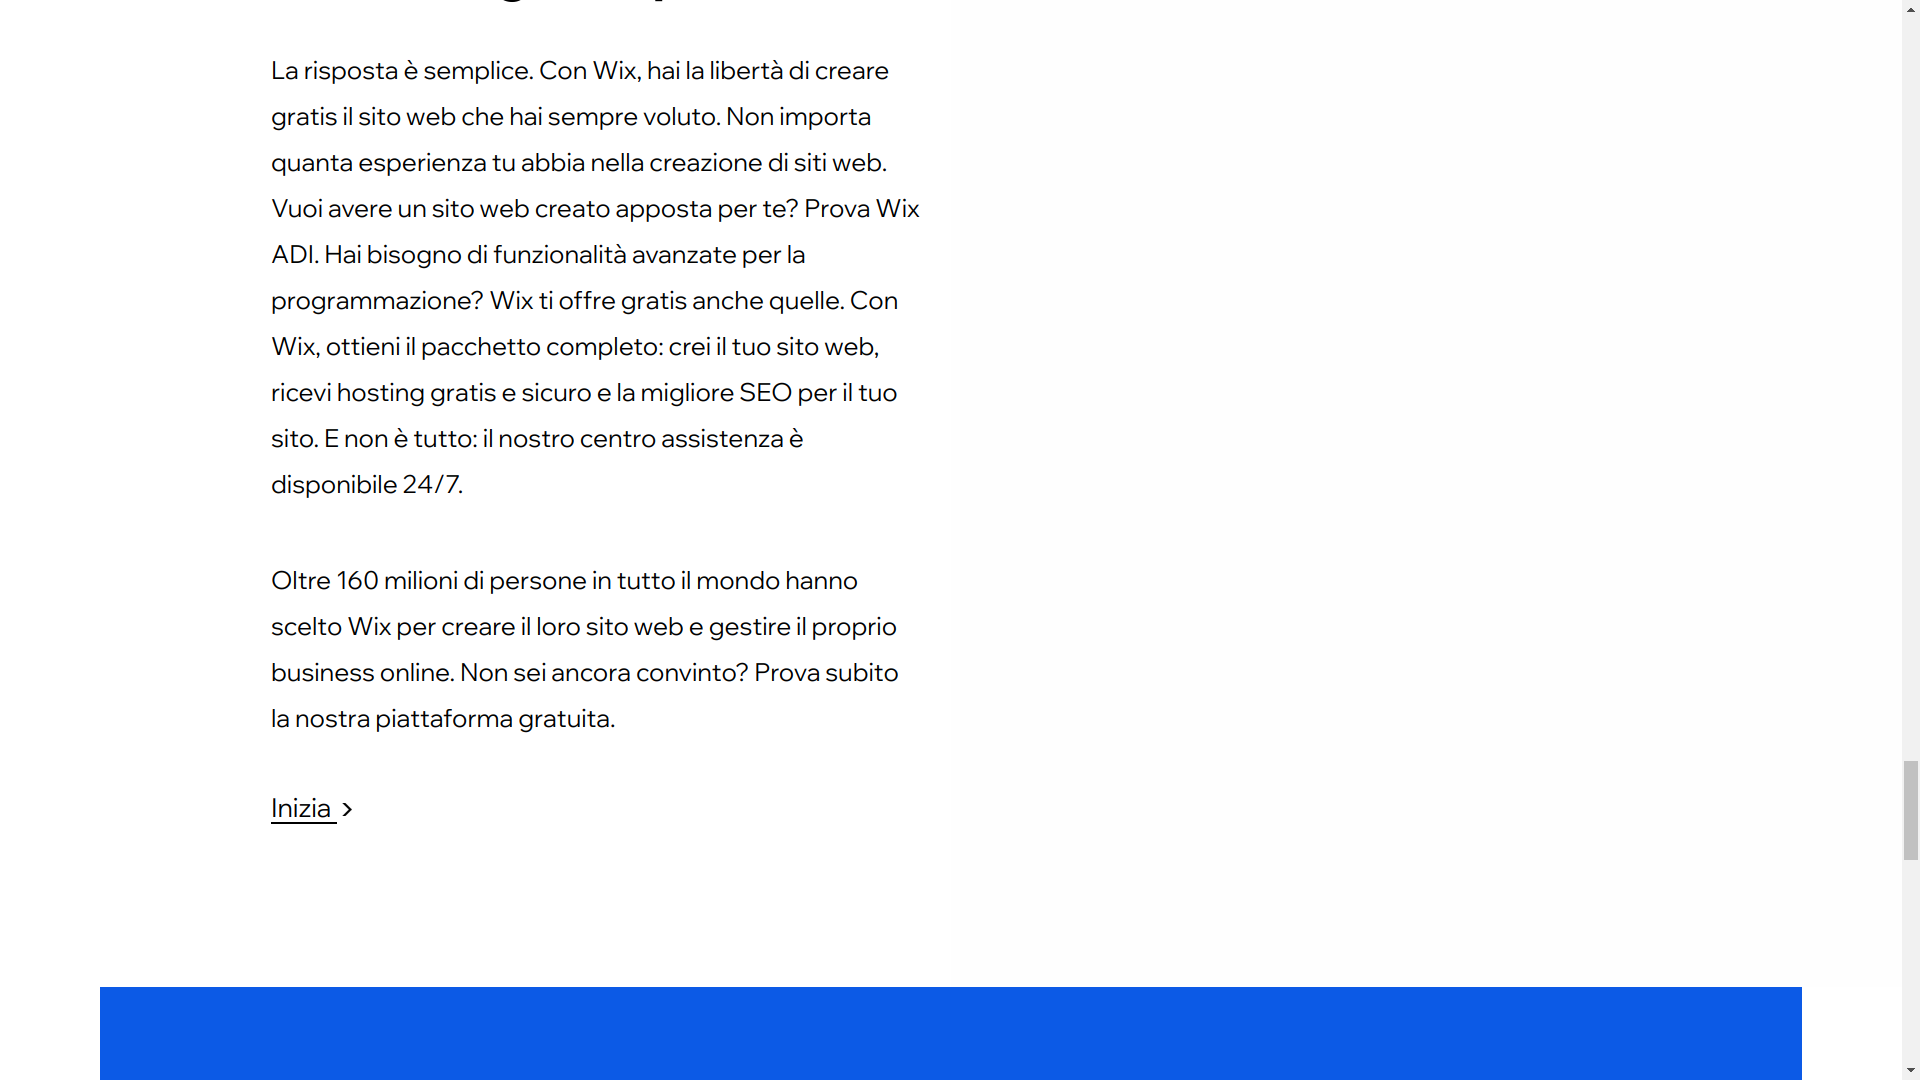
\includegraphics[width=1\textwidth]{img/homepage-09.png}
  \caption{Homepage (pt. 9)}
  \label{fig:homepage-09}
\end{figure}

La scheramata \ref{fig:homepage-10} mostra passo per passo gli step da
seguire per ``Creare gratis un sito web'', come recita il titolo.

\begin{figure}[H]
  \centering
  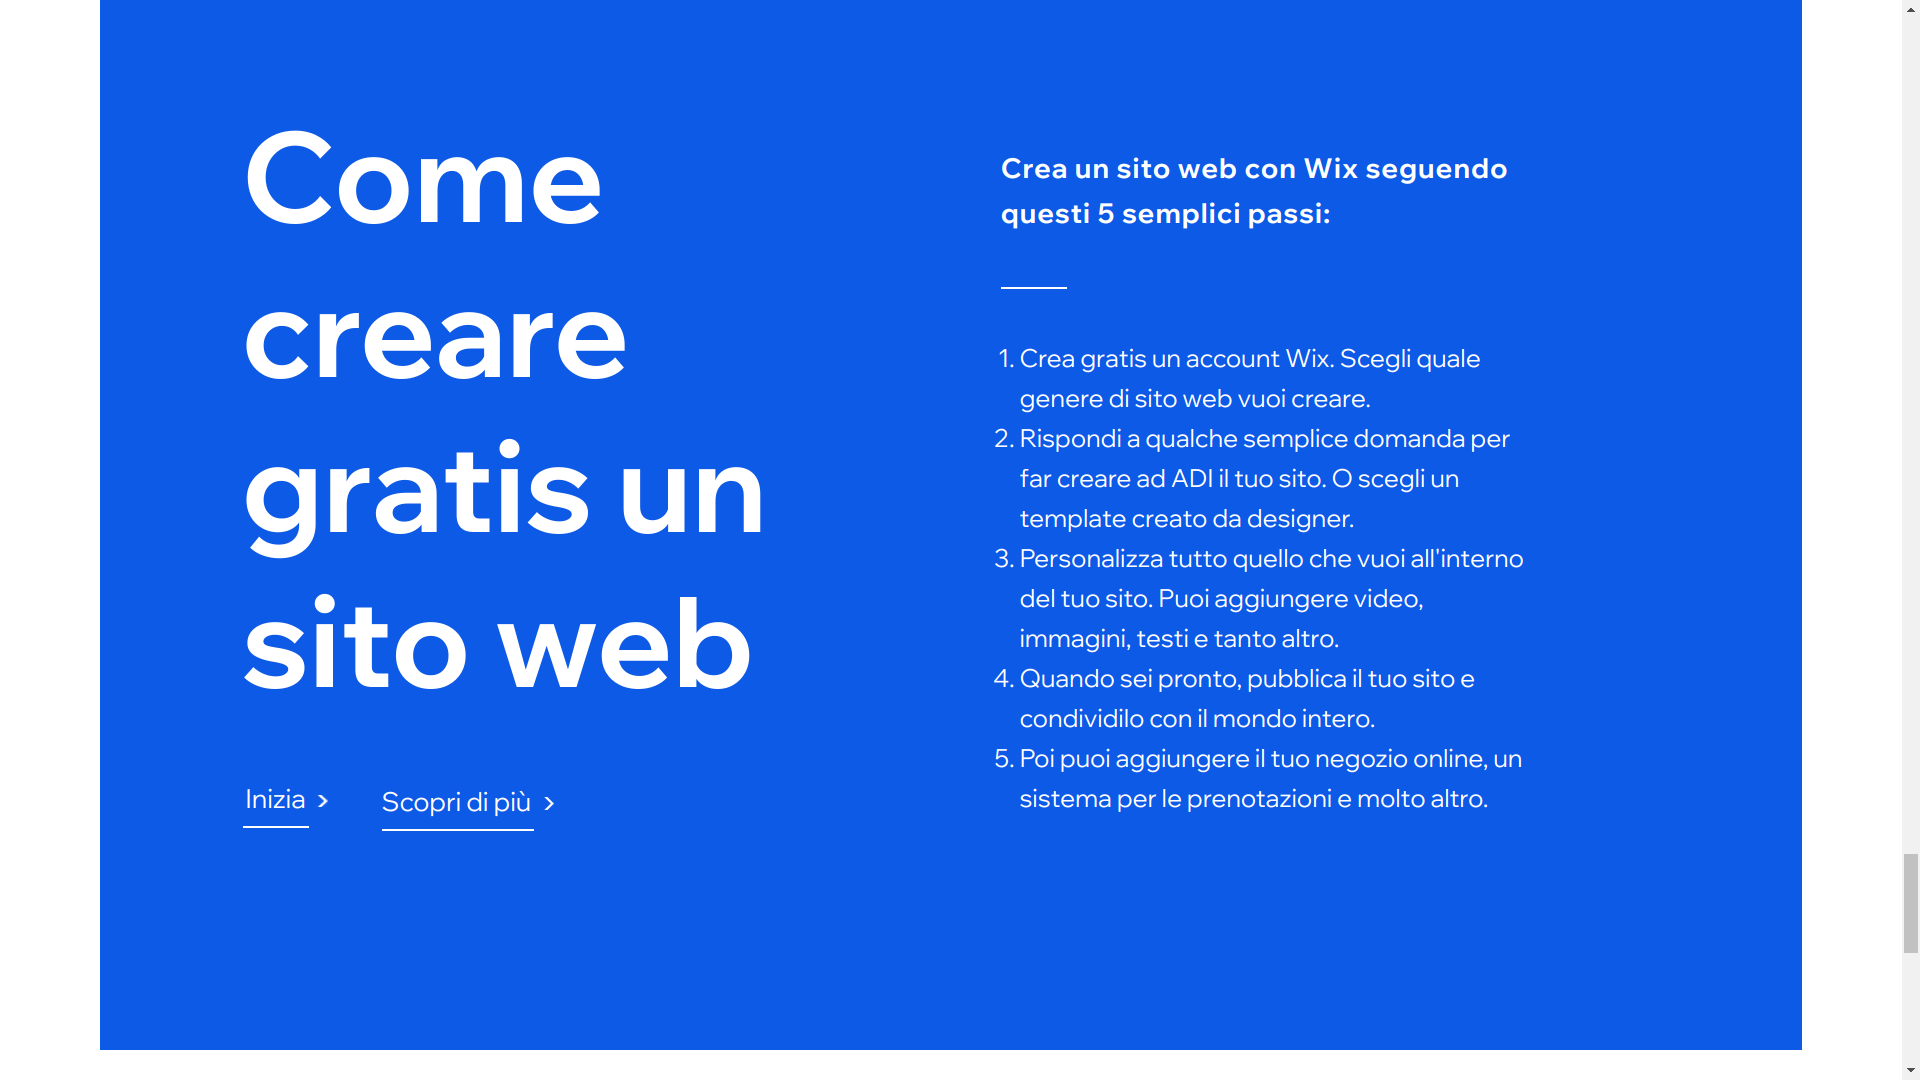
\includegraphics[width=1\textwidth]{img/homepage-10.png}
  \caption{Homepage (pt. 10)}
  \label{fig:homepage-10}
\end{figure}

Con la schermata \ref{fig:homepage-11} finalmente si conclude la
homepage. Sono forniti diversi link a prodotti correlati, informazioni
sull'azienda e riferimenti al supporto.

\begin{figure}[H]
  \centering
  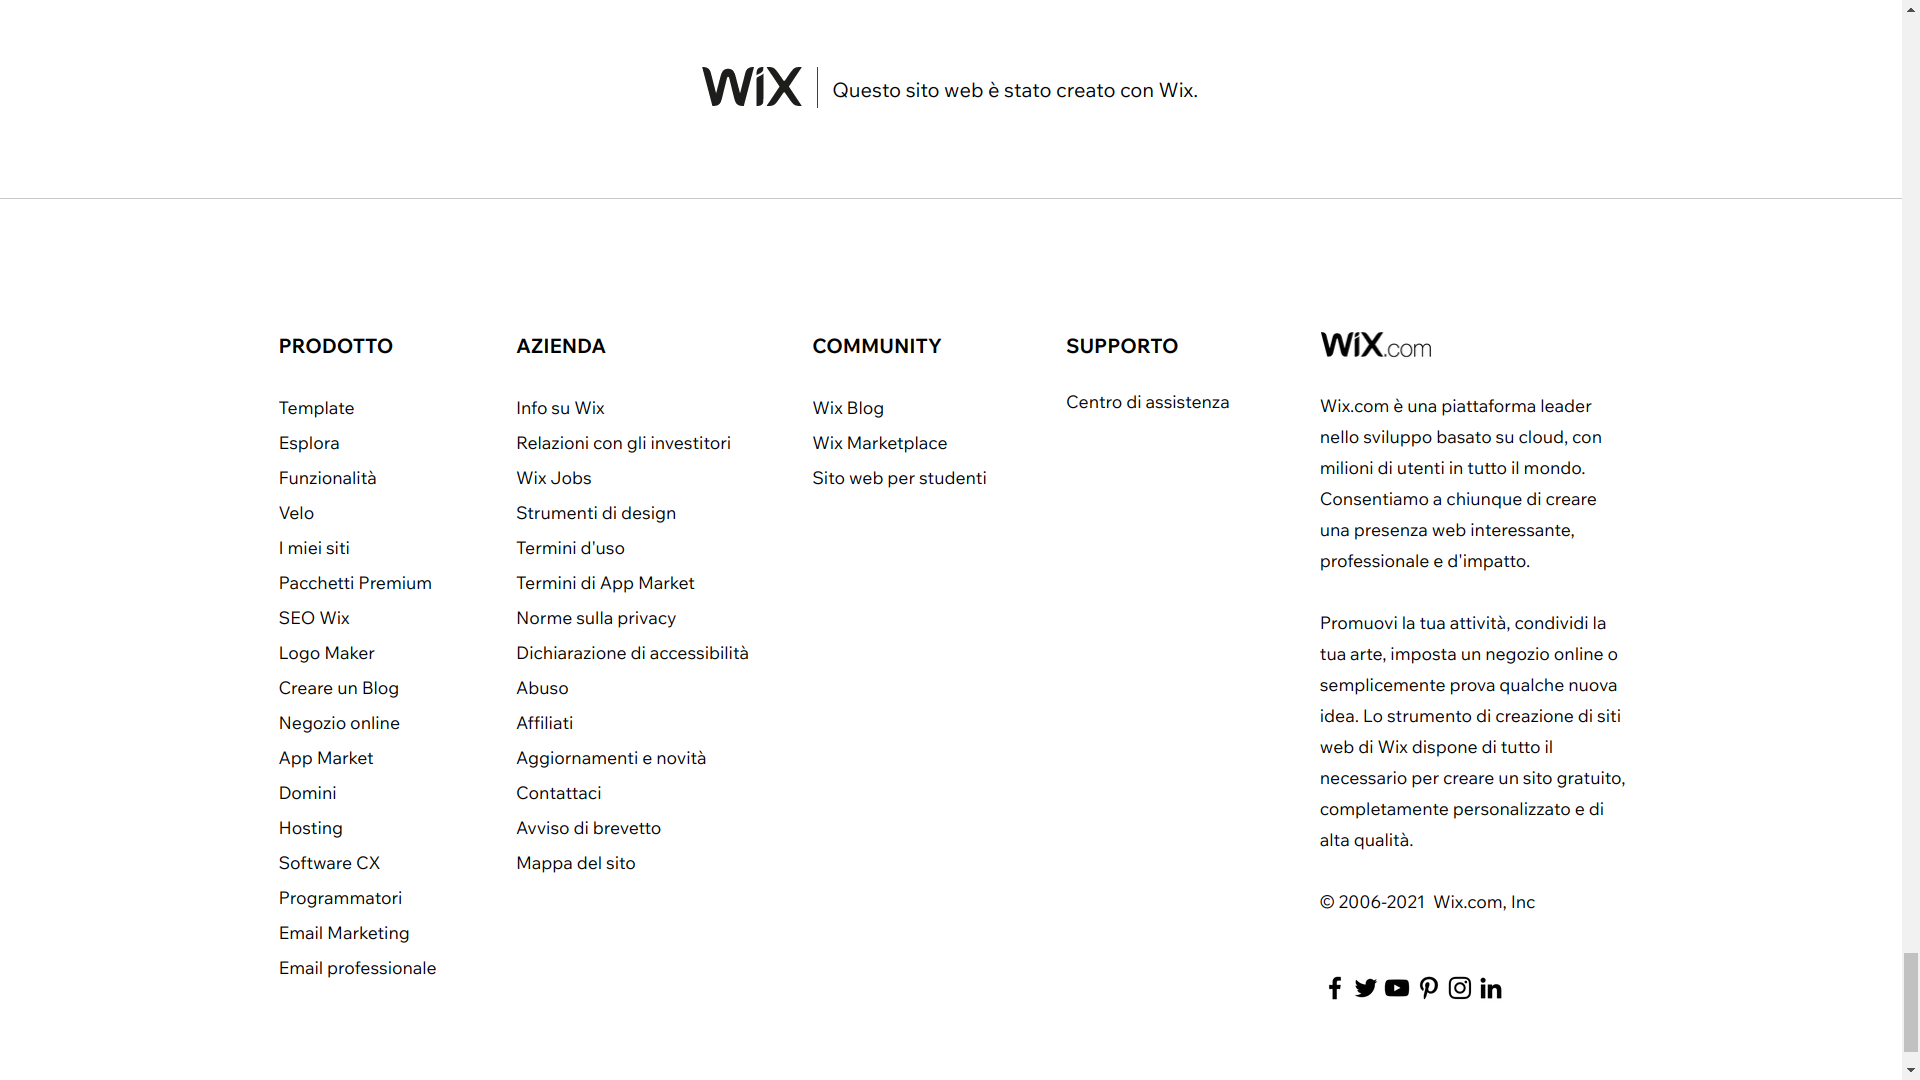
\includegraphics[width=1\textwidth]{img/homepage-11.png}
  \caption{Homepage (pt. 11)}
  \label{fig:homepage-11}
\end{figure}

\subsection{The Six Ws}
\label{subsec:homepage-the-six-ws}

\section{Pagina interna: Funzionalità}
\label{sec:secondary-page-analysis}

\subsection{Descrizione generale}
\label{subsec:internalpage-description}

\subsection{The Six Ws}
\label{subsec:internalpage-the-six-ws}

\section{Analisi complessiva}
\label{sec:full-analysis}

\subsection{Struttura}
\label{subsec:structure}

\subsection{Navigazione}
\label{subsec:navigation}

\subsection{Pubblicità}
\label{subsec:ads}

\subsection{Immagini}
\label{subsec:images}

\subsection{Registrazione}
\label{subsec:signup}

\section{Altre pagine}
\label{sec:other-pages}

\section{Considerazioni finali}
\label{sec:final-remarks}

\section{Giudizio finale}
\label{sec:final-vote}

\end{document}
